%%%%%%%%%%%%%%%%%%%%%%%%%%%%%%%%%%%%%%%%%
% Article EcoFoG
% Version 2.1 (23/10/2017)
%
% adapté de :
% Stylish Article
% LaTeX Template
% Version 1.0 (31/1/13)
%
% This template has been downloaded from:
% http://www.LaTeXTemplates.com
%
% Original author:
% Mathias Legrand (legrand.mathias@gmail.com)
%
% License:
% CC BY-NC-SA 3.0 (http://creativecommons.org/licenses/by-nc-sa/3.0/)
%
%%%%%%%%%%%%%%%%%%%%%%%%%%%%%%%%%%%%%%%%%


%----------------------------------------------------------------------------------------
%	PACKAGES AND OTHER DOCUMENT CONFIGURATIONS
%----------------------------------------------------------------------------------------

\documentclass[fleqn,10pt]{ArtEcoFoG} % Document font size and equations flushed left

\setcounter{tocdepth}{3} % Show only three levels in the table of contents section: sections, subsections and subsubsections


% Pandoc environments
\usepackage{framed}
\usepackage{fancyvrb}
\providecommand{\tightlist}{%
  \setlength{\itemsep}{0pt}\setlength{\parskip}{0pt}}
\newcommand{\VerbBar}{|}
\newcommand{\VERB}{\Verb[commandchars=\\\{\}]}
\DefineVerbatimEnvironment{Highlighting}{Verbatim}{commandchars=\\\{\}, fontsize=\scriptsize} % Code R
\definecolor{shadecolor}{RGB}{248,248,248}
\newenvironment{Shaded}{\begin{snugshade}}{\end{snugshade}}
\newcommand{\KeywordTok}[1]{\textcolor[rgb]{0.13,0.29,0.53}{\textbf{{#1}}}}
\newcommand{\DataTypeTok}[1]{\textcolor[rgb]{0.13,0.29,0.53}{{#1}}}
\newcommand{\DecValTok}[1]{\textcolor[rgb]{0.00,0.00,0.81}{{#1}}}
\newcommand{\BaseNTok}[1]{\textcolor[rgb]{0.00,0.00,0.81}{{#1}}}
\newcommand{\FloatTok}[1]{\textcolor[rgb]{0.00,0.00,0.81}{{#1}}}
\newcommand{\ConstantTok}[1]{\textcolor[rgb]{0.00,0.00,0.00}{{#1}}}
\newcommand{\CharTok}[1]{\textcolor[rgb]{0.31,0.60,0.02}{{#1}}}
\newcommand{\SpecialCharTok}[1]{\textcolor[rgb]{0.00,0.00,0.00}{{#1}}}
\newcommand{\StringTok}[1]{\textcolor[rgb]{0.31,0.60,0.02}{{#1}}}
\newcommand{\VerbatimStringTok}[1]{\textcolor[rgb]{0.31,0.60,0.02}{{#1}}}
\newcommand{\SpecialStringTok}[1]{\textcolor[rgb]{0.31,0.60,0.02}{{#1}}}
\newcommand{\ImportTok}[1]{{#1}}
\newcommand{\CommentTok}[1]{\textcolor[rgb]{0.56,0.35,0.01}{\textit{{#1}}}}
\newcommand{\DocumentationTok}[1]{\textcolor[rgb]{0.56,0.35,0.01}{\textbf{\textit{{#1}}}}}
\newcommand{\AnnotationTok}[1]{\textcolor[rgb]{0.56,0.35,0.01}{\textbf{\textit{{#1}}}}}
\newcommand{\CommentVarTok}[1]{\textcolor[rgb]{0.56,0.35,0.01}{\textbf{\textit{{#1}}}}}
\newcommand{\OtherTok}[1]{\textcolor[rgb]{0.56,0.35,0.01}{{#1}}}
\newcommand{\FunctionTok}[1]{\textcolor[rgb]{0.00,0.00,0.00}{{#1}}}
\newcommand{\VariableTok}[1]{\textcolor[rgb]{0.00,0.00,0.00}{{#1}}}
\newcommand{\ControlFlowTok}[1]{\textcolor[rgb]{0.13,0.29,0.53}{\textbf{{#1}}}}
\newcommand{\OperatorTok}[1]{\textcolor[rgb]{0.81,0.36,0.00}{\textbf{{#1}}}}
\newcommand{\BuiltInTok}[1]{{#1}}
\newcommand{\ExtensionTok}[1]{{#1}}
\newcommand{\PreprocessorTok}[1]{\textcolor[rgb]{0.56,0.35,0.01}{\textit{{#1}}}}
\newcommand{\AttributeTok}[1]{\textcolor[rgb]{0.77,0.63,0.00}{{#1}}}
\newcommand{\RegionMarkerTok}[1]{{#1}}
\newcommand{\InformationTok}[1]{\textcolor[rgb]{0.56,0.35,0.01}{\textbf{\textit{{#1}}}}}
\newcommand{\WarningTok}[1]{\textcolor[rgb]{0.56,0.35,0.01}{\textbf{\textit{{#1}}}}}
\newcommand{\AlertTok}[1]{\textcolor[rgb]{0.94,0.16,0.16}{{#1}}}
\newcommand{\ErrorTok}[1]{\textcolor[rgb]{0.64,0.00,0.00}{\textbf{{#1}}}}
\newcommand{\NormalTok}[1]{{#1}}
\usepackage{longtable,booktabs}
\usepackage{caption}
% These lines are needed to make table captions work with longtable:
\makeatletter
\def\fnum@table{\tablename~\thetable}
\makeatother
% longtable 2 columns
% https://tex.stackexchange.com/questions/161431/how-to-solve-longtable-is-not-in-1-column-mode-error
\makeatletter
\let\oldlt\longtable
\let\endoldlt\endlongtable
\def\longtable{\@ifnextchar[\longtable@i \longtable@ii}
\def\longtable@i[#1]{\begin{figure}[t]
\onecolumn
\begin{minipage}{0.5\textwidth}\scriptsize
\oldlt[#1]
}
\def\longtable@ii{\begin{figure}[t]
\onecolumn
\begin{minipage}{0.5\textwidth}\scriptsize
\oldlt
}
\def\endlongtable{\endoldlt
\end{minipage}
\twocolumn
\end{figure}}
\makeatother

\usepackage{graphicx,grffile}
\makeatletter
\def\maxwidth{\ifdim\Gin@nat@width>\linewidth\linewidth\else\Gin@nat@width\fi}
\def\maxheight{\ifdim\Gin@nat@height>\textheight0.8\textheight\else\Gin@nat@height\fi}
\makeatother
% Scale images if necessary, so that they will not overflow the page
% margins by default, and it is still possible to overwrite the defaults
% using explicit options in \includegraphics[width, height, ...]{}
\setkeys{Gin}{width=\maxwidth,height=\maxheight,keepaspectratio}

% User-adder preamble
\usepackage{textcomp} \usepackage{tabu} \usepackage{caption}
\captionsetup{justification = justified}
\renewenvironment{table}{\begin{table*}}{\end{table*}\ignorespacesafterend}
\hyphenation{bio-di-ver-si-ty sap-lings re-or-gan-i-za-tion post-dis-tur-bance dis-tur-bance}
\usepackage[left]{lineno} \linenumbers \usepackage{bookmark}

%----------------------------------------------------------------------------------------
%	ARTICLE INFORMATION
%----------------------------------------------------------------------------------------

\JournalInfo{\ }
\Archive{\ }

\PaperTitle{Diverging taxonomic and functional trajectories following disturbance in
a Neotropical forest} % Article title

\Authors{
Ariane MIRABEL\textsuperscript{1*}\\ Bruno Herault\textsuperscript{2}\\ Eric Marcon\textsuperscript{1}
} % Authors
\affiliation{
\textsuperscript{1}UMR EcoFoG, AgroParistech, CNRS, Cirad, INRA, Université des Antilles,
Université de Guyane.\\ \hspace{1em} Campus Agronomique, 97310 Kourou, France.\\\textsuperscript{2}INPHB, Institut National Polytechnique Félix Houphoüet-Boigny\\ \hspace{1em} Yamoussoukro, Ivory Coast.
}
\affiliation{*\textbf{Corresponding author}: ariane.mirabel@gmail.com, https://github.com/ArianeMirabel} % Corresponding author

\Keywords{Community Ecology, Disturbance Trajectories, Intermediate Disturbance Hypothesis, Mid-term Resilience, Neotropical Forests, Taxonomic and Functional Biodiversity} % Keywords - if you don't want any simply remove all the text between the curly brackets
\newcommand{\keywordname}{Keywords} % Defines the keywords heading name

%----------------------------------------------------------------------------------------
%	ABSTRACT
%----------------------------------------------------------------------------------------

\Abstract{
In the current global change context, it is urgent to anticipate the
fate of tropical forests. This means understanding tree community
response to disturbance and the underlying processes. In that respect,
we aim here to clarify taxonomic and functional post-disturbance
trajectories, and determine the scope of the Intermediate Disturbance
Hypothesis (IDH) that remains debated in tropical forests.
\color{black}We analyzed community trajectories following a disturbance
gradient from 10 to 60\% of above-ground biomass loss in a Neotropical
forest over 30 years.\color{red} We considered trajectories along time
of community taxonomic and functional trajectories in terms of richness,
evenness, composition, and redundancy. We based on the annual botanical
inventories of 75 ha of a Neotropical forest and on large trait datasets
comprising seven leaf, stem, and life-history traits. We identified a
decoupling between taxonomic composition, differing among communities,
and functional composition, \color{red} similar among communities and
convergent in the functional space.\color{black} \color{red} The
taxonomic diversity followed humped-shaped trajectories along time after
disturbance depending on the initial disturbance intensity, which
validated the IDH (Intermediate Disturbance Hypothesis).\color{black}
The functional diversity trajectories,however, were homogeneous among
plots and dismissed the IDH. We explained this decoupling by the
variations in community functional redundancy that mitigated the
functional impact of disturbance. Although consistent, the recovery of
community composition, diversity, and redundancy remained unachieved
after 30 years. \color{red} These results acknowledged the need of
decades-long cycles without disturbance to ensure community complete
recovery.\color{black}
}

%----------------------------------------------------------------------------------------

\begin{document}

\selectlanguage{english}

\flushbottom % Makes all text pages the same height

\maketitle % Print the title and abstract box

\tableofcontents % Print the contents section

\thispagestyle{empty} % Removes page numbering from the first page

%----------------------------------------------------------------------------------------
%	ARTICLE CONTENTS
%----------------------------------------------------------------------------------------
























\section{Introduction}\label{introduction}

The large areas covered with tropical forests worldwide hold crucial
environmental, economic, and social values. They provide wood and
multiple non-timber forest products, shelter a diversified fauna, and
ensure cultural and human well-being. They regulate local and regional
climates, as well as carbon, water and nutrient cycles. However, the
growing demand in forests products together with current global changes
increase the pressure on remaining undisturbed forests
\citep{Morales-Hidalgo2015}. \color{red}These threats may change the
frequency and magnitude of the natural disturbance regime that defines
and maintains the structure, composition, and functioning of tree
communities \citep{Schnitzer2001, Anderson-Teixeira2013, Sist2015}.
\color{black} To anticipate the fate of tropical forests, it is urgent
to understand tree community response to disturbance, and the underlying
ecological processes. The forest cover is generally maintained following
disturbance, but modifications in the fluxes of light, heat, and water
\citep{Goulamoussene2017} change community abiotic and biotic
environments. These changes translate into post-disturbance community
trajectories that have been largely studied through trajectories of
forest structural parameters such as aboveground biomass, tree height or
stem density \citep{Piponiot2016, Rutishauser2016}. Some of the
determinants of post-disturbance biomass trajectories are already
identified, like the structure and composition of the pre-disturbance
community, or the post-disturbance environmental parameters
\citep{Herault2018}. Community diversity and composition trajectories,
however, have not been as thoroughly understood
\citep{Guitet2018, Molino2001}, and manifold biodiversity trajectories
might emerge given the variety of species response to disturbance and
the diversity of tropical forests
\citep{Lindenmayer2012, Garcia_florez2017}.

An early conceptual basis of the linkage between biodiversity and
disturbance is the Intermediate Disturbance Hypothesis (IDH). The IDH
states a relationship between the community diversity and the intensity
and frequency of disturbance events, and postulates a diversity peak at
intermediate level of disturbance \citep{Connell1978}. This is based on
the fluctuations of community environment following disturbance that
foster both competitively superior species and fast colonizers, and
prevents competitive exclusion \citep{Shea2004, Pulsford2016}.
\color{red} In tropical forests, some studies advocate community
deterministic response to disturbance, as for example in the dry and wet
forests in Ghana \citep{Bongers2009} or in the guianese rainforests
\citep{Molino2001}, where intermediate disturbance proved to increase
the community richness by increasing the proportion of pioneers or
heliophilous species in the community while maintaining the richness in
old-growth forest species. In other cases, however, observations of the
IDH diverge from theoretical expectations
\citep{Hugues2007, Sheil2003, Norden2017}. Some studies refute the role
of disturbance intensity, as observed in forest gaps in Panama where no
difference in species richness was found between forest gaps and
undisturbed areas \citep{Hubbell2001}, or in costa-rican forests where
forests that did not follow deterministic convergence display stochastic
trajectories \citep{Norden2015}.\\
The high diversity of tropical forests may foster the emergence of
numerous facilitation, adaptation, and inter- and intra-specific
competition following disturbance
\citep{Garcia_florez2017, Bongers2009}.These interactions can result in
miscellaneous responses to disturbance \citep{Lindenmayer2012}, which
question the validity of the IDH in tropical forests
\citep{Hubbell2001, Fox2013, Sheil2013}. \color{black}

Analysing community response to disturbance and grasp all aspects of
community changes requires a wide array of metrics
\citep{Sheil2003, Shea2004, Mayfield2010}. The analysis should first
consider community composition, which is crucial for conservation issues
and reveals the pool of species fostered or hampered by disturbance
\citep{Lavorel2002, Bellwood2006}. This should be completed with
diversity metrics encompassing both community richness and evenness to
assess the changes in community abundance distribution. Besides,
functional approaches have been shown to usefully complement pure
taxonomic approaches as they shed light on the species biological
attributes directly linking community diversity, composition, and
redundancy to ecosystem functioning \citep{Violle2007b, Baraloto2012a}.
In that respect, a vast literature allowed recognizing major traits
representing species ecological strategy and determining how they
respond to changing conditions \citep{Diaz2005}. Specifically, in
tropical forests, the functional approach revealed the emergence of
deterministic processes following disturbance. Such deterministic
processes entailed a shift from a dominance of ``conservative''
slow-growing species dealing with scarce resources, to a dominance of
``acquisitive'' fast-growing species with rapid and efficient use of
abundant resources \citep{Rees2001, Reich2014, Herault2011}. This shift
is translated into the trajectories of average community value of key
functional traits related to resource acquisition, as leaf and stem
traits, and life-history strategy, as seed mass and maximum size
\citep{Wright2004, TerSteege2006, Westoby2006a, Chave2009b}.

The functional approach also encompasses the analysis of functional
redundancy, that quantifies the amount of shared trait values among
species \citep{Carmona2016}. The typical high functional redundancy of
hyper-diverse tropical forests \citep{Bellwood2006} mitigates the
impacts of species removal on ecosystem functioning, and determines
community resilience after disturbance \citep{Elmqvist2003, Diaz2005}.

Here, we monitored over 30 years the response of 75 ha of Neotropical
forest plots set up on a gradient of disturbance intensity, from 10 to
60\% of above-ground biomass (AGB) loss. We made use of a large
functional traits database encompassing major leaf, stem, and
life-history traits in order to draw the taxonomic and functional
trajectories in terms of richness, evenness, composition, and
redundancy. Specifically, (i) we drew taxonomic and functional
post-disturbance trajectories and examined the underlying ecological
processes, (ii) we discussed the scope of the IDH regarding taxonomic
and functional facets of community diversity, and (iii) we analyzed
community resilience and time to recovery. \color{red} We hypothesized
that community functional and taxonomic trajectories might not track
each other, given the high functional redundancy in tropical forests.
While functional diversity would be enhanced by the environmental
changes following disturbance, specifically the increase in light
availability, taxonomic trajectories would only increase until a
disturbance intensity threshold, as pioneers recruited following
disturbance are not as diverse as late-successional species. Community
taxonomic and functional would hence follow different rates of recovery.
\color{black}

\section{Material and Methods}\label{material-and-methods}

\subsection{Study site}\label{study-site}

Paracou station in French Guiana (5° 18'N and 52° 53'W) is located in a
lowland tropical rain forest in a tropical wet climate with mean annual
temperature of 26° C, and mean annual precipitation averaging 2980
mm.y\textsuperscript{-1} (30-y period). The climate comprises a 3-month
dry season (\textless{} 100 mm.month\textsuperscript{-1}) from
mid-August to mid-November, and a one-month dry season in March
\citep{Wagner2011}. Across all plots, elevation ranges from 5 to 50 m,
and the topography mainly corresponds to hilltops or hillsides, while
bottomlands cover less than 1 \% of the area. Plots are shallow
ferralitic acrisols over a layer of transformed saprolite with low
permeability and lateral drainage. Soil conditions are homogeneous, to
the exception of the highest hilltops where the thick surface allows a
free vertical drainage \citep{Gourlet-Fleury2004}.

The experiment is a network of twelve 6.25 ha plots\color{red},
distributed over a 400ha area \color{black}(Table \ref{tab:Tab1}, Supp.
Mat. Fig. S1), that undergone three disturbance treatments in 1987
according to a randomized plot design \citep{Gourlet-Fleury2004}.\\
\color{red}The experiment intended to simulate logging intensities and
distinguished the treatments for non-commercial commercial species,
logged at 40cm DBH to simulate thinning operations.\color{black} The
experiment comprised three replicates of three sylvicultural treatments
(hereafter plots T1, T2, and T3), and three control plots (T0).
\color{red}Control plots are set in mature forest stand that did not
undergone any logging nor intense anthropic activities activities for
the last 500 years\color{black}. All treatments T1, T2, and T3 comprised
the logging of 10 trees/ha with 50 cm minimum DBH that belonged to a set
of 58 commercially exploited species \citep{Gourlet-Fleury2004}.
Treatment T2 additionally comprised a thinning treatment by
poison-girdling of non-commercially exploited species randomly selected
with an average of 30 trees/ha with 40 cm minimum DBH. Treatment T3
additionally comprised the logging of 15 trees/ha with 40 cm minimum
DBH, and the poison-girdling of 20 trees/ha with a 50 cm minimum DBH,
all belonging to non-commercially exploited species. Considering the
silvicultural treatments and the following damage, disturbance intensity
was measured as the percentage of aboveground biomass (\%AGB) lost
between the first inventory in 1984 and five years after disturbance
\citep{Piponiot2016} estimated with the BIOMASS R package
\citep{Rejou2017}. \color{red} Tree diameter are provided in the
experimental dataset, wood density is extracted from global wood density
(GWD) database \citep{Zanne2009}, and tree height is retrieved from a
generic H--D model based on a single bioclimatic predictor (eqn 6a in
\citep{Chave2014}). The AGB is measured from the generalized allometric
model eqn 4 of \citep{Chave2014}. \color{black} The three treatments
were then transformed into a continuous disturbance intensity gradient
with increasing above-ground biomass (AGB) loss.

\begin{table}

\caption{\label{tab:Tab1}Intervention table, summary of the disturbance intensity for the 4 plot treatments in Paracou. Treatment intensities are defined by the minimum logging DBH (Diameter at Breast Height), the type of logged species (commercially exploited or not), the density of logged trees, and the total AGB (Above Ground Biomass) lost after treatment.}
\centering
\begin{tabu} to \linewidth {>{\raggedright}X>{\raggedright}X>{\raggedright}X>{\raggedright}X>{\raggedright}X}
\toprule
Treatment & Timber & Thinning & Fuelwood & \%AGB lost\\
\midrule
Control & - & - & - & 0\\
T1, low & DBH $\geq$ 50 cm, commercially exploited species, $\approx$ 10   $trees.ha^{-1}$ & - & - & $[12-33]$\\
T2, intermediate & DBH $\geq$ 50 cm, commercially exploited species, $\approx$ 10  $trees.ha^{-1}$ & DBH $\geq$ 40 cm, non-commercially exploited species, $\approx$ 30   $trees.ha^{-1}$ & - & $[33-56]$\\
T3, high & DBH $\geq$ 50 cm, commercially exploited species, $\approx$ 10  $trees.ha^{-1}$ & DBH $\geq$ 50 cm, non-commercially exploited species, $\approx$ 15  $trees.ha^{-1}$ & 40 cm $\leq$ DBH $\leq$ 50 cm, non-commercially exploited species,\ $\approx$ 15 $trees.ha^{-1}$ & $[35-56]$\\
\bottomrule
\end{tabu}
\end{table}

\subsection{Inventories protocol and dataset
collection}\label{inventories-protocol-and-dataset-collection}

The study site corresponds to a tropical rainforest typical of the
Guiana Shield with a dominance of Fabaceae, Chrysobalanaceae,
Lecythidaceae, and Sapotaceae. In the 12 experimental plots, all trees
above 10 cm DBH have been mapped and measured annually since 1984. Trees
are first identified with a vernacular name assigned by the forest
worker team, and afterward with a scientific name assigned by botanists
during regular botanical campaigns. In 1984, specific vernacular names
were given to 62 commmon or commercially exploited species. More
infrequent species were identified under general identifiers only
distinguishing trees and palms. From 2003, botanical campaigns have been
conducted every 5 to 6 years to identify all trees at the species level.
In 2015, however, identification levels still varied among plots and
campaigns.

This variability of protocols in time raised methodological issues as
vernacular names usually correspond to various botanical species. This
resulted in significant taxonomic uncertainty that had to be accounted
for in the measure of composition and diversity metrics. Uncertainty
propagation was implented within a Bayesian framework using
vernacular/botanical names associations to reconstitute complete
inventories at genus level from real incomplete ones. Vernacular names
were replaced through multinomial trials based on the association
probability \(\big[\alpha_1, \alpha_2,..., \alpha_V\big]\) observed
across all inventories between each vernacular name \emph{v} and all
species \(\big[s_1, s_2,..., s_N\big]\):

\begin{align}
M_v\Big(\big[s_1, s_2,..., s_N\big],\big[\alpha_1, \alpha_2,..., \alpha_V\big]\Big) \nonumber
\end{align}

See Supplementary Materials -Fig. S2 and \citet{Aubry-Kientz2013} for
the detailed methodology.

Six functional traits representing the leaf economics (\emph{i.e.} leaf
thickness, toughness, total chlorophyll content, and specific leaf
area), and the stem economics (\emph{i.e.} wood specific gravity and
bark thickness) were obtained from the BRIDGE project \footnote{http://www.ecofog.gf/Bridge/}.
Trait values were assessed from a selection of individuals located in
nine permanent plots in French Guiana, including two in Paracou, and
comprised 294 species belonging to 157 genera. Whenever a species was in
the dataset but missed some trait values (10\% of the species), missing
values were filled using multivariate imputation by chained equation
\citep{Mice2011}. To account for the phylogenetic signal in the
imputation process, imputations were based on samples of species from
the same genus or from the same family. Whenever a species was not in
the dataset, it was attributed a set of trait values randomly sampled
among species of the next higher taxonomic level (same genus or family).
Two life-history traits, maximum specific height and seed mass, came
from the Mariwenn database \footnote{https://www.ecofog.gf/mariwenn/}.
The database compiles information from a vast literature on the flora of
French Guiana \citep{Ollivier2007} and comprises 362 species belonging
to 188 genera. As seed mass information was classified into classes, no
data filling process was applied and analyses were restricted to the
botanical species recorded.

\color{red}Confidence intervals of the composition and diversity metrics
were computed after 50 iterations of the uncertainty propagation
framework.\color{black}

\subsection{Composition and diversity
metrics}\label{composition-and-diversity-metrics}

Because of the variable precision of botanical identification efforts,
we had to conduct the taxonomic composition and diversity analysis at
the genus level. \color{red}Functional composition, diversity, and
redundancy measures were conducted at species level.\color{black}
Taxonomic and functional trajectories of community composition were
drawn in a two-dimensional NMDS ordination plane. Two NMDS using
abundance-based (\emph{i.e.} Bray-Curtis) dissimilarity measures were
conducted to map either taxonomic or functional composition, the latter
based on the seven leaf, stem, and life history traits (without seed
mass classes). Trajectories along time were reported through the
Euclidean distance between the target inventories and the 1984
pre-disturbance inventories of reference. Univariate trajectories of the
leaf, stem, and life-history traits were also visualized with the
community weighted means (CWM) \citep{Diaz2007}. Species seed mass were
given in 5 mass classes, and seed mass trajectories were reported as the
proportion of each class in the inventories (Supplementary materials).

The taxonomic and functional trajectories were analysed from the 1984
pre-disturbance inventories of reference. The taxonomic diversity was
reported through species richness and the Hill number translation of the
Simpson index \citep{Hill1973}. The comparison between these two metrics
assesses community taxonomic richness and evenness: thereafter, results
will be discussed directly in terms of taxonomic richness and evenness.
Both indices are recommended for diversity studies \citep{Marcon2015},
and belong to the set of \color{red} Tsallis or generalized entropy
\color{black} corresponding, respectively, to the 0 and 2 order of
diversity (q). \color{red}Diversity metrics were measured using the Hqz
function from the entropart package \citep{Marcon2015}.\color{black} The
functional diversity was reported using the functional richness and
functional evenness. \color{red}Both functional richness and evenness
were measured through a distance-based dissimilarity matrix built with
the daisy function of the cluster R package \citep{Cluster2019}, using
the Gower distance between species, similar to \citet{Herault2007a},
\citet{Herault2007b}.\color{black} The functional diversity was measured
through the Rao index of quadratic entropy. The Rao index combines the
community abundance distribution\color{red}, from species relative
abundance, \color{black} and the average pairwise functional
dissimilarity between species computed by the Gower distance.
\color{red}The comparison between these two metrics assesses community
functional richness and evenness: thereafter, results will be discussed
directly in terms of functional richness and evenness.\color{black}

The impacts of the initial disturbance levels on the maximum gain or
loss in richness and evenness were tested with the Spearman rank
correlation tests. Richness and evenness trajectories were besides
analyzed through polynomial regression \color{red}or simple linear
models \color{black} between (i) taxonomic and functional richness and
evenness, and (ii) the initial \%AGB loss at 10, 20, and 30 years after
disturbance. \color{red}The best model fitting, between linear or
quadratic model, was chosen based on their respective AIC criterion. The
explanatory power of the fit were measured to adjusted r-square
values.\color{black}

Finally, functional redundancy was measured as the overlap among species
in community functional space \citep{Carmona2016}. First, the
individuals of the trait database were mapped in the plane of the first
two axes from a PCA analysis. The PCA analysis lowered the weight of
correlations among traits as the axes are combinations of the most
decoupled traits. \color{red}The two main PCA axis respectively hold
26\% and 19\% of the trait dataset variance.\color{black} For each
species, the traits probability density (TPD) were computed from the
mapping of individuals through two-dimension kernel density estimators.
\color{red} We used the kde2d function of the MASS package
\citep{MASS2002} that is a gaussian density estimator for a
2-dimensional space. \color{black} Second, for each community, the TPD
weigthed by species abundance were summed across the functional space.
Third, the functional space was divided into a 100 x 100 grid, and the
number of species with a positive TPD was counted in each cell. The
average count across cells minus 1 returned the Community Functional
Redundancy, which was the average number of species in the community
that share the same trait values.

\section{Results}\label{results}

\subsection{Community Composition}\label{community-composition}

From 1984, the first pre-disturbance inventory, to 2015, 28 years after
disturbance, 828 388 individual trees and 591 botanical species spanning
223 genera and 64 families were recorded.

In undisturbed plots, both taxonomic and functional composition remained
stable (Fig. \ref{fig:NMDSplans}). In disturbed plots, both trajectories
followed marked and consistent trajectories over time.

The functional composition trajectory resembled, in disturbed
communities, to cyclic compositional changes with an incomplete recovery
of the initial composition (Fig.\ref{fig:NMDSplans}). The maximum
dissimilarity with the initial state was positively correlated with the
disturbance intensity for both taxonomic and functional composition
(\(\rho_{Spearman}^{Taxonomic}=0.94\) and
\(\rho_{Spearman}^{Functional}=0.90\), respectively. Fig.
\ref{fig:SumUp}). The maximum dissimilarity with the initial state was
reached for taxonomic composition between 15 to 25 years, and between 20
to 25 years for functional composition.

\begin{figure*}

{\centering 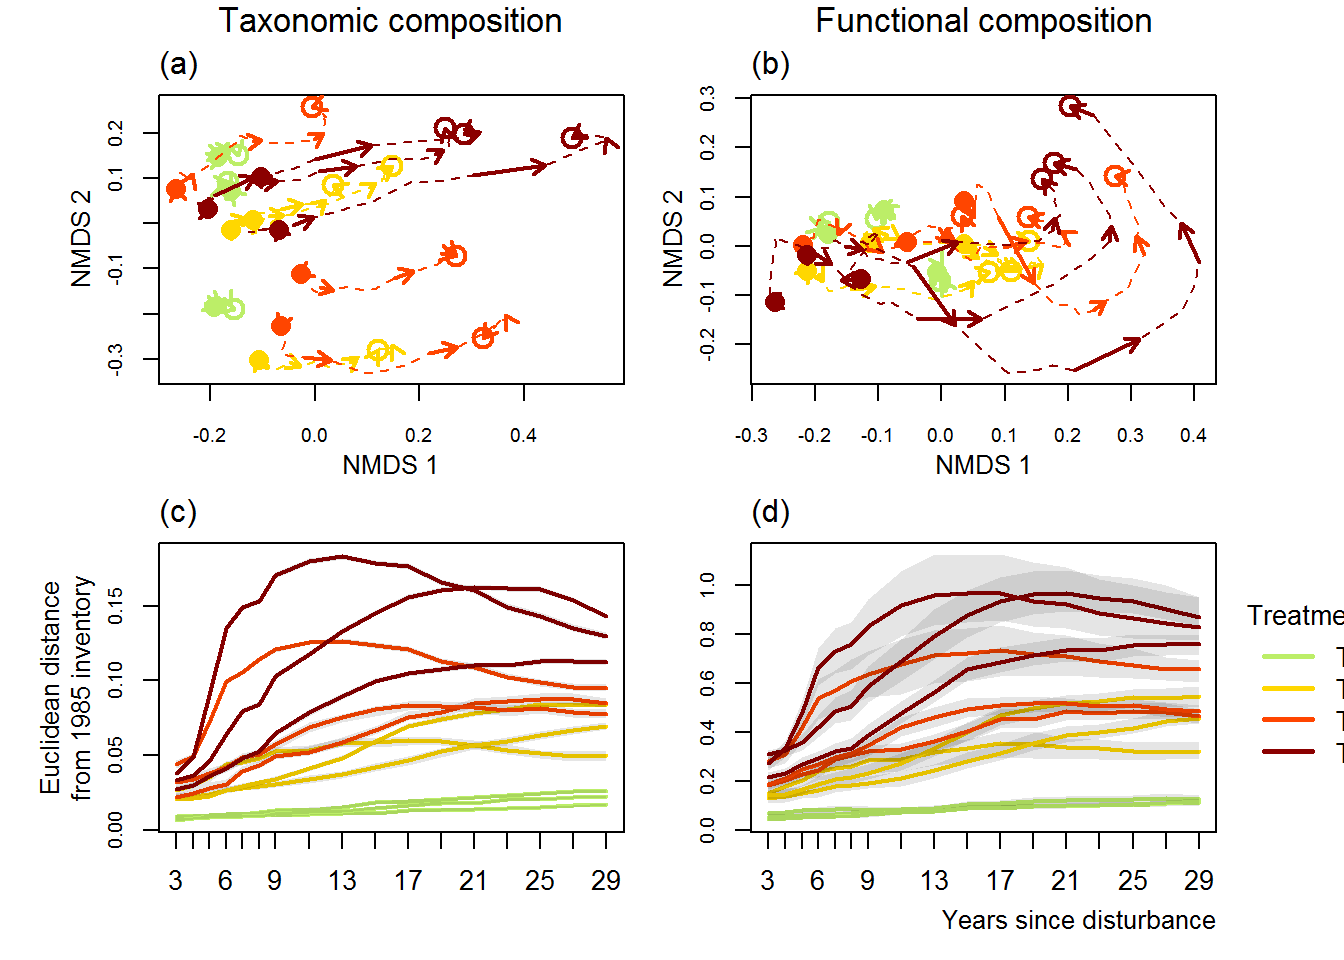
\includegraphics[width=1\linewidth]{WholePlotTrajectories_files/figure-latex/NMDSplans-1} 

}

\caption{Plot trajectories in terms of taxonomic composition (\textbf{(a)} and \textbf{(c)}), and functional composition (\textbf{(b)} and \textbf{(d)}) in a two-dimensional NMDS plane. Lower panels (\textbf{(c)} and \textbf{(d)}) represent the Euclidean distance to initial condition along the 30 sampled years. Shaded areas are the credibility intervals.}\label{fig:NMDSplans}
\end{figure*}

In control plots, Community Weighted Means (CWM) of functional traits
remained stable in time.\\
In disturbed plots, they mostly followed unimodal trajectories, either
stabilizing or returning towards their initial values, to the exception
of leaf chlorophyll content, which continued to increase 30 years after
disturbance for 4 out of 6 highly disturbed plots. \color{red}Main
tendencies for disturbed plots were a decrease followed by a slight
increase of maximum height at adult stage (\emph{Hmax}), leaf toughness,
and wood specific gravity (\emph{WSG}), but trait values remained
significantly lower than their initial value (Fig. \ref{fig:CWM}).
\color{black} Bark thickness and specific leaf area (\emph{SLA}) both
increased along time. Bark thickness remained substantially high after
30 years, and \emph{SLA} had almost recovered to its initial value.
Whatever the functional traits, the maximum difference to initial value
was highly correlated to the disturbance intensity. \color{red}Positive
correlations were observed for leaf thickness, chlorophyll content, SLA
and bark thickness (\(\rho_{Spearman}^{Leaf thickness}=0.79\),
\(\rho_{Spearman}^{Chlorophyll content}=0.61\),
\(\rho_{Spearman}^{SLA}=0.99\),
\(\rho_{Spearman}^{Bark thickness}=0.68\)). Maxima were observed between
5 and 15 years following disturbance for leaf thickness and SLA while
chlorophyll content and bark thickness kept increasing after 30 years
for leaf chlorophyll content and bark thickness. Negative correlation
was observed for leaf toughness, WSG, and Hmax
(\(\rho_{Spearman}^{Leaf toughness}=-0.47\),
\(\rho_{Spearman}^{WSG}=-0.80\), \(\rho_{Spearman}^{Hmax}=-0.28\)).
Minima were observed between 5 and 15 years following disturbance for
Hmax, 10 and 20 years for WSG, and between 15 and 25 years following
disturbance for leaf toughness.\color{black} The proportions of the
three lightest seed mass classes increased in all disturbed plots. After
30 years the proportion of lightest seed mass class decreased while it
stabilized for the two other lightest seed mass classes (Supp. Mat. -
Fig. S3).

\begin{figure*}

{\centering 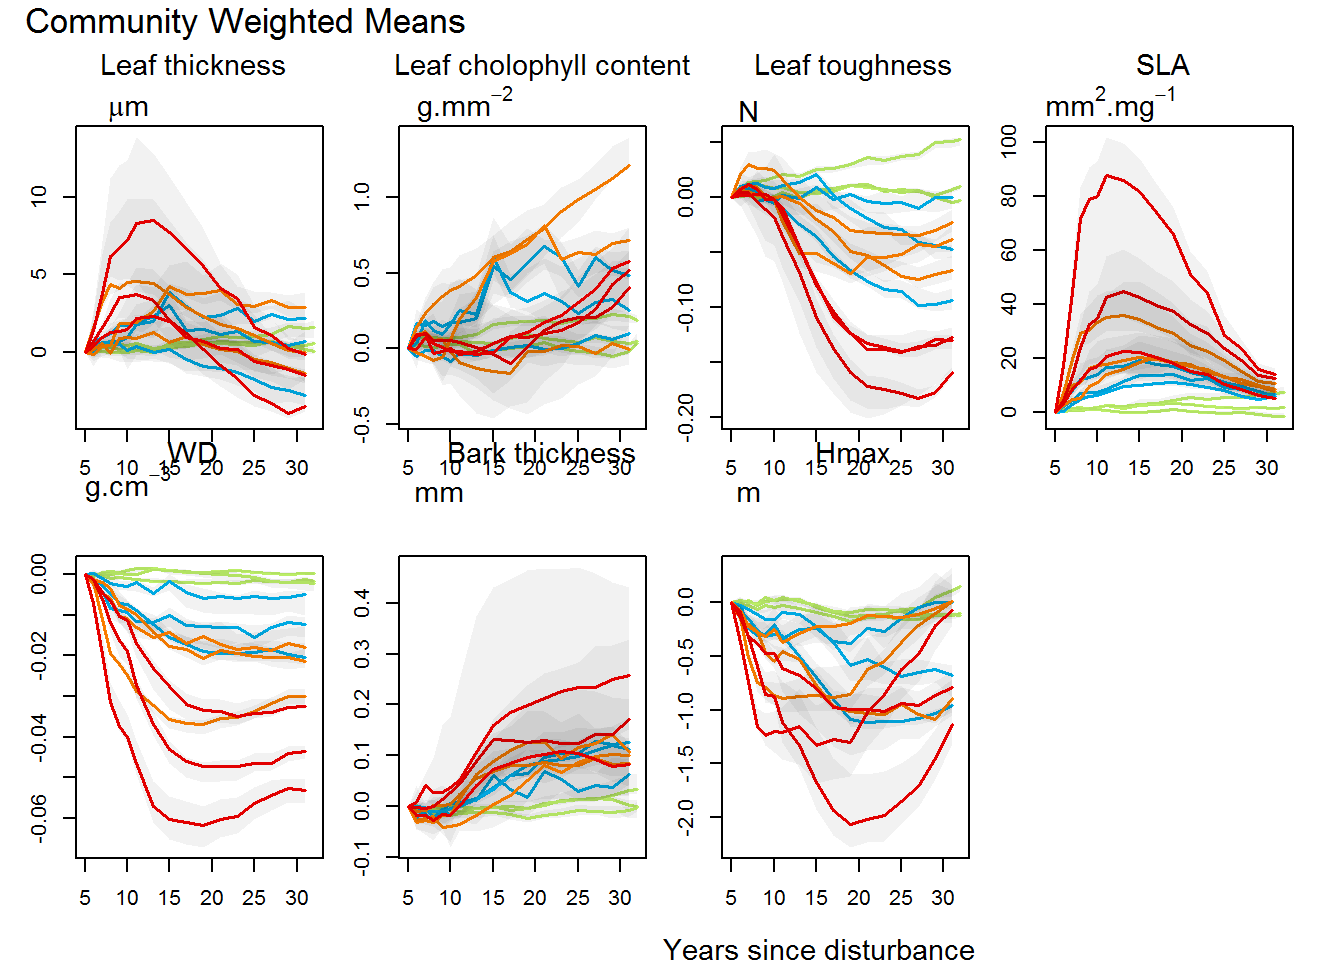
\includegraphics[width=1\linewidth]{WholePlotTrajectories_files/figure-latex/CWM-1} 

}

\caption{Trajectories of community weighted means over 30 years after disturbance of four leaf traits (leaf thickness, chlorophyll content, toughness, and specific area), two stem traits (wood specific gravity and bark thickness), and one life history trait (species maximum height at adult stage). }\label{fig:CWM}
\end{figure*}

\subsection{Community taxonomic and functional
diversity}\label{community-taxonomic-and-functional-diversity}

Taxonomic richness and evenness remained stable in control plots over
the 30 years of monitoring. In disturbed communities, after low
disturbance intensity the taxonomic richness increased, reaching a
maximum gain of 14 botanical genera. After intense disturbance the
taxonomic richness followed a more complex trajectory, decreasing for
ten years after disturbance before recovering to pre-disturbance values.
\color{red}The maximum rate of change compared to initial richness was
positively correlated with the disturbance intensity
(\(\rho_{Spearman}^{Richness}=0.73\)).\color{black}

In all disturbed plots \color{red}, to the exception of plots 5 (T2) and
12 (T3) that showed a small initial drop, \color{black} the evenness
first increased until a maximum reached after around 20 years. This
maximum was positively correlated with the disturbance intensity
(\(\rho_{Spearman}^{Evenness}=0.82\), \color{red} Fig.
\ref{fig:SumUp})\color{black}. The evenness then stabilized except for
two intensively-disturbed plots (number 8 and 12) for which it kept
increasing (Fig. \ref{fig:DivTaxo}).

\begin{figure*}

{\centering 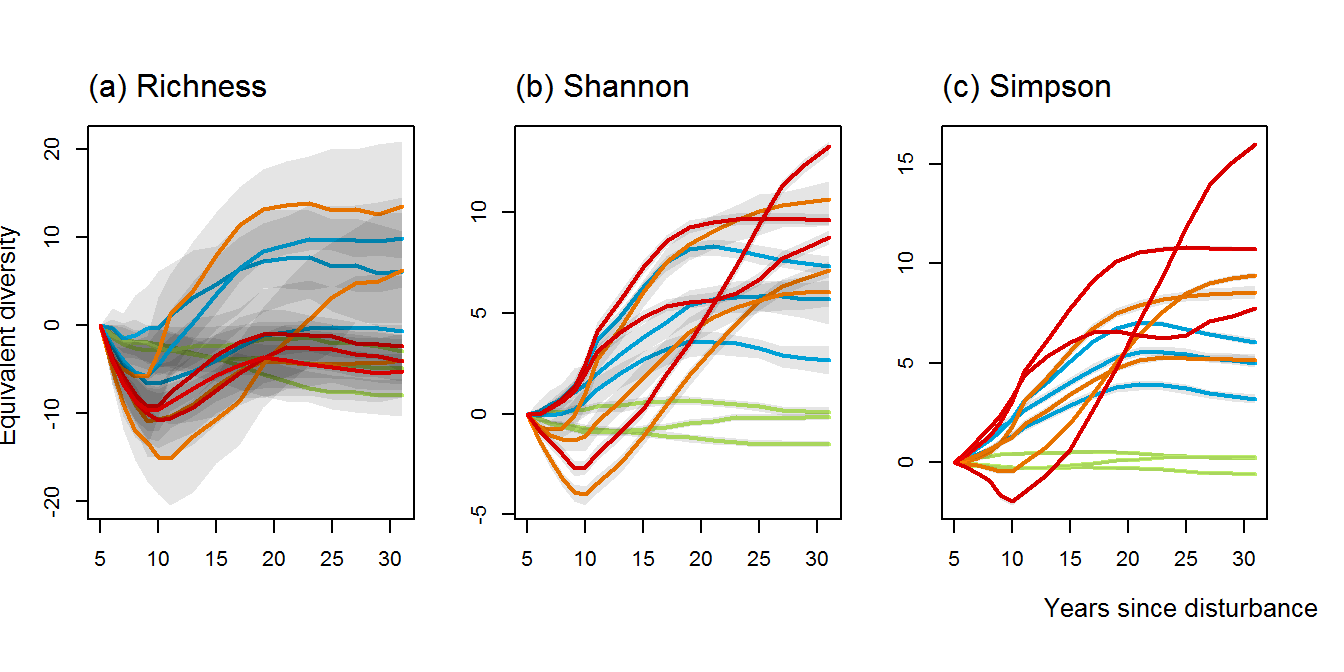
\includegraphics[width=1\linewidth]{WholePlotTrajectories_files/figure-latex/DivTaxo-1} 

}

\caption{Trajectories of community taxonomic richness \textbf{(a)}, taxonomic evenness, \textbf{(b)}, functional richness \textbf{(c)}, and functional evenness \textbf{(d)}. Values correspond to the difference over 30 years of community diversity with the values of 1989 inventories of reference, 5 years after disturbance. Shaded areas are the credibility intervals }\label{fig:DivTaxo}
\end{figure*}

Functional richness and evenness remained stable in control plots over
the 30 years of monitoring. \color{red}In disturbed communities, both
functional richness and evenness trajectories increased following
disturbance, with maxima positively correlated to \%AGB loss
\(\rho_{Spearman}^{Richness} = 0.76\) and
\(\rho_{Spearman}^{Evenness} = 0.60\) (Fig. \ref{fig:SumUp}).
\color{black} For low \color{red}and intermediate
\color{black}disturbance intensity, functional richness and evenness
displayed a low but long-lasting increase up to a maximum reached after
20-25 years. For high disturbance intensity, they generally displayed a
fast but short increase followed, after 10 years, by a slow decrease
towards the initial values.

The second-degree polynomial regressions between (i) the percentage AGB
loss, and (ii) the taxonomic and functional diversity showed various
shapes depending on the diversity indices and on the time since
disturbance (Fig. \ref{fig:IDHplot}). \color{red}Regarding taxonomic
diversity, the taxonomic richness showed a humped-shaped trajectory with
the disturbance intensity, and peaked at 20\% of initial AGB loss. The
relationship between disturbance intensity and taxonomic evenness,
however, was humped-shaped only 20 years after disturbance and linear
for 10 and 30 years after disturbance times.\color{black} Regarding
functional diversity, \color{red} the relationship was linear for both
taxonomic richness and evenness, except for the functional diversity
after 30 years. \color{black}

\begin{figure*}

{\centering 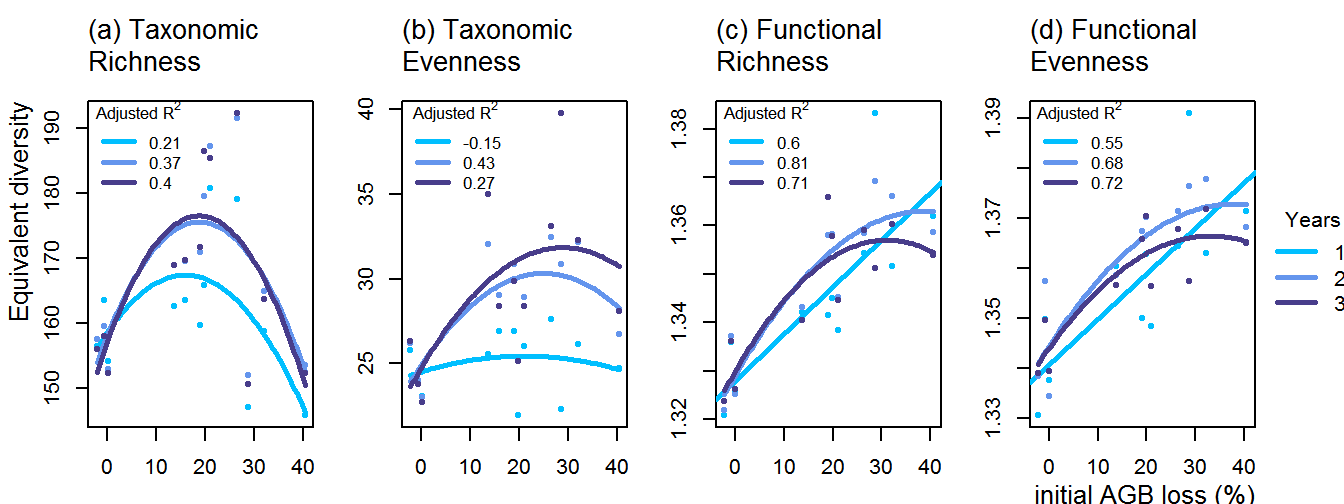
\includegraphics[width=1\linewidth]{WholePlotTrajectories_files/figure-latex/IDHplot-1} 

}

\caption{Relationship between the initial \%AGB loss and community taxonomic richness \textbf{(a)}, taxonomic evenness \textbf{(b)}, functional richness \textbf{(c)}, and functional evenness \textbf{(d)} at 10, 20, and 30 years after disturbance.}\label{fig:IDHplot}
\end{figure*}

\subsection{Functional redundancy}\label{functional-redundancy}

Control plots displayed stable functional redundancy over time. All
disturbed plots had lower functional redundancy than control plots and
followed similar humped-shaped trajectories (Fig. \ref{fig:RedFunRest}).
The maximum redundancy loss was positively correlated with the
disturbance intensity (\(\rho_{Spearman}=0.31\), (Fig. \ref{fig:SumUp}))
and the recovery trajectory had not attained initial values for any
disturbed communities after 30 years.

\begin{figure}

{\centering 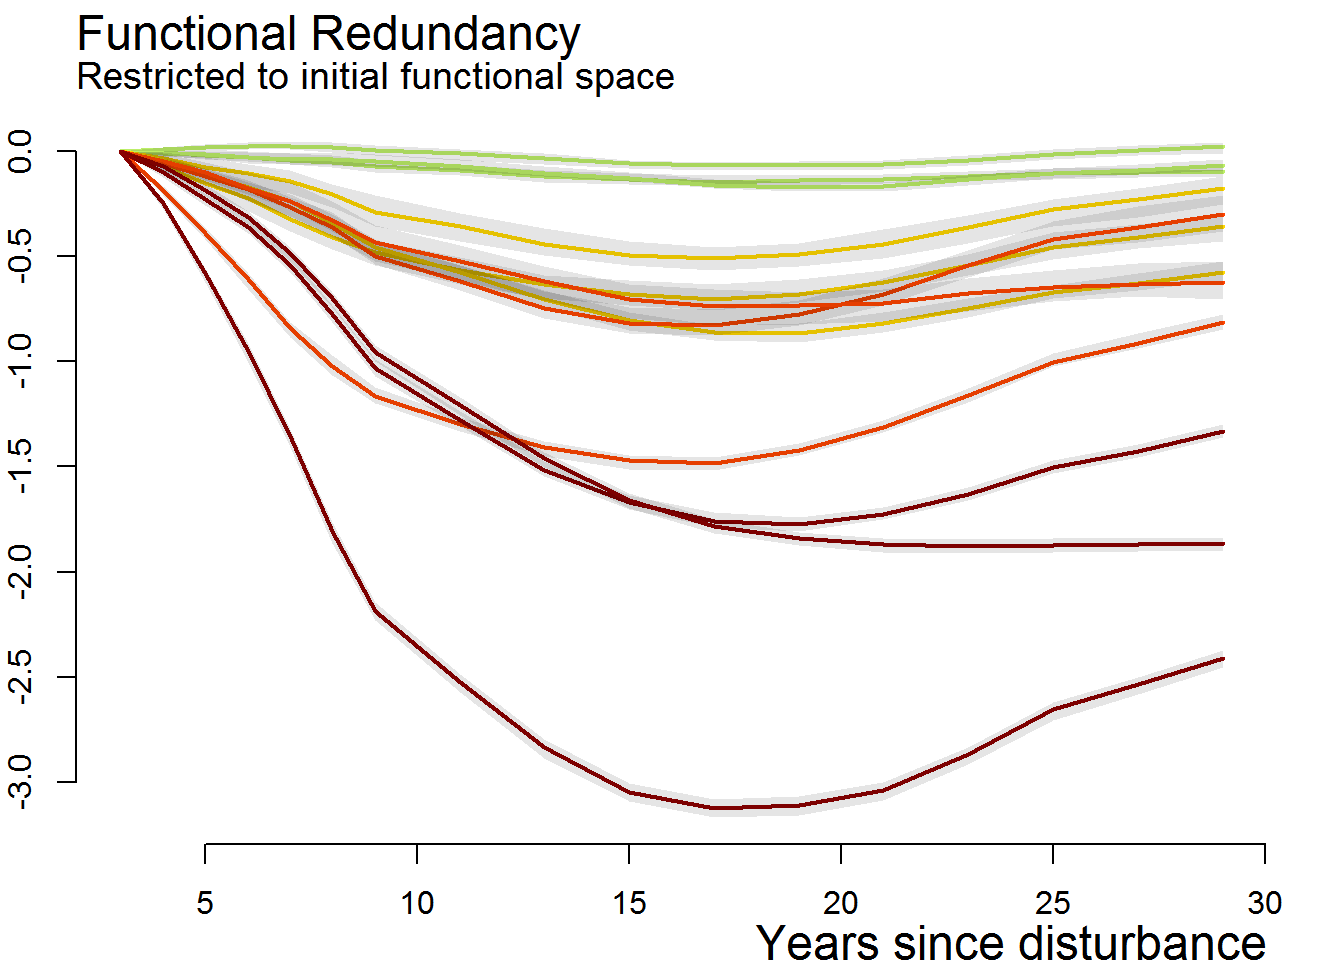
\includegraphics[width=0.4\linewidth]{WholePlotTrajectories_files/figure-latex/RedFunRest-1} 

}

\caption{Trajectories of the functional redundancy within the initial functional space over 30 years after disturbance. The redundancy is measured in a two-dimensional plan summarizing 45\% of species variance in the functional space of the 7 leaf, stem, and life history traits. Redundancy value represent the average number of species in the community that share the same trait values. Shaded areas are the credibility intervals.}\label{fig:RedFunRest}
\end{figure}

\begin{figure}

{\centering 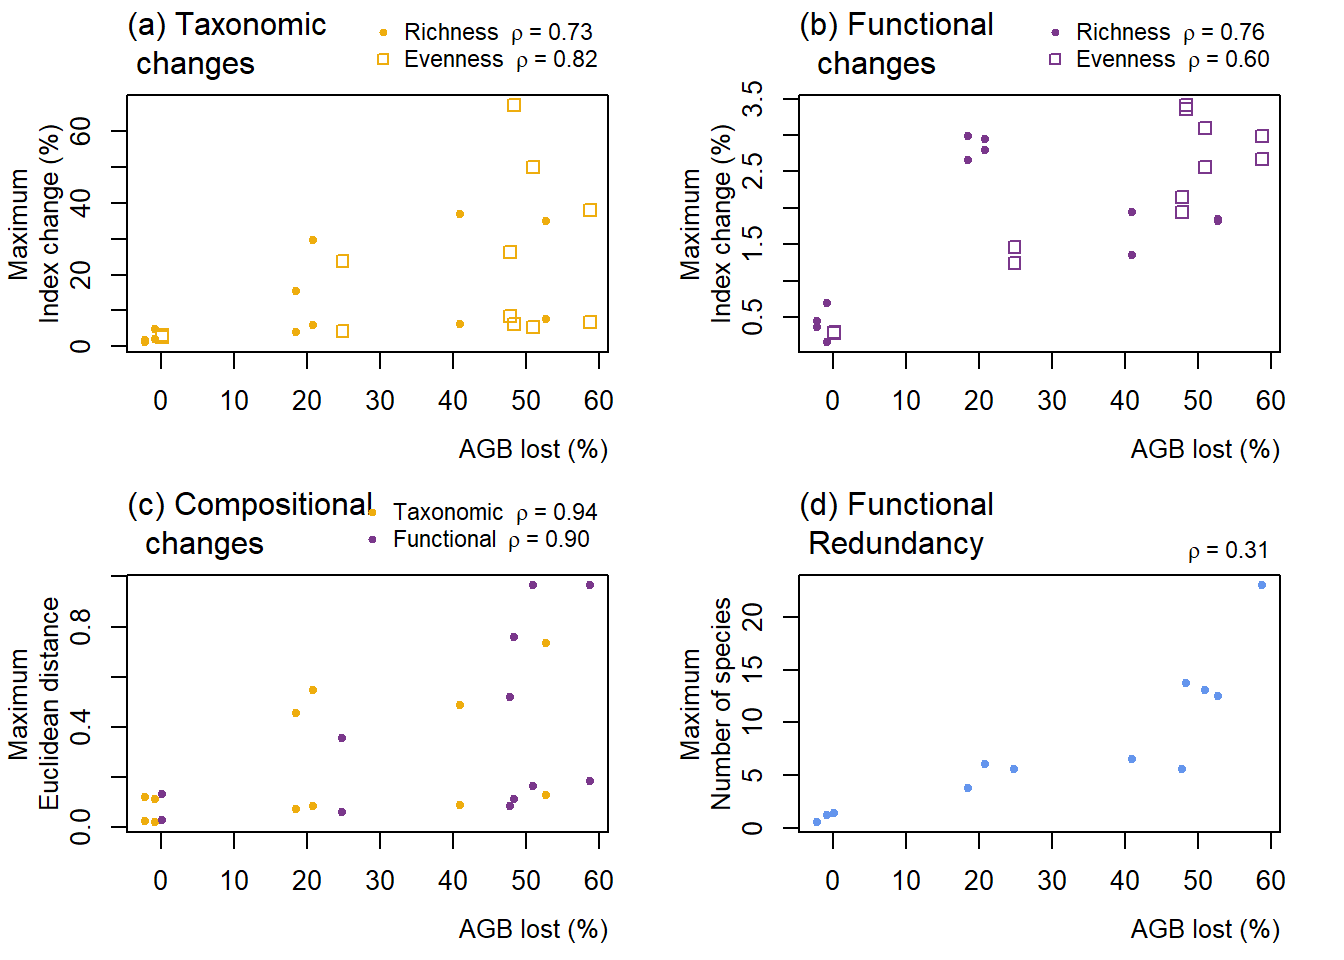
\includegraphics[width=1\linewidth]{WholePlotTrajectories_files/figure-latex/SumUp-1} 

}

\caption{Maximum changes in taxonomic and functional diversity and composition against disturbance intensity, expressed as percentage of initial disturbance. Upper panels display taxonomic richness and evenness \textbf{(a)}, and functional richness and evenness \textbf{(b)} expressed in percentage of change compared to initial value. Lower panels display taxonomic and functional euclidean distance from pre-disturbance inventory, respectively in the spaces of species and functional traits \textbf{(c)}, and functional redundancy expressed as number of redundant species in the community \textbf{(d)}.}\label{fig:SumUp}
\end{figure}

\section{Discussion}\label{discussion}

\color{red}Our analysis revealed that community post-disturbance
trajectories in taxonomic and functional diversity and composition were
decoupled. The taxonomic composition specificities between communities
before disturbance were maintained following disturbance, while their
functional composition converged in the functional space. \color{black}
In terms of diversity, only the taxonomic trajectories validated the IDH
that explained humped-shaped post-disturbance trajectories whith an
amplitude depending on the disturbance intensity. The decoupling between
taxonomic and functional response \color{red} could be
\color{black}explained by variations in community functional redundancy.
\color{red}The loss of species or the changes in their abundance would
impact the taxonomic but not the functional diversity and composition,
as redundant species with the same functional characteristics remain in
the community. The trajectory of the functional redundancy hence
appeared determinant for community recovery.\color{black}

\subsection{Decoupled taxonomic and functional
trajectories}\label{decoupled-taxonomic-and-functional-trajectories}

\color{red}From pre-disturbance to 30 years after disturbance,
communities showed different location along NMDS axis 2 that hardly
changed along time. Specificities in community taxonomic composition,
materialized by the distinct location on the NMDS axis 2, existed before
disturbance. The disturbance led a displacement on the NMDS axis 1
only.\color{black} Taxonomic \color{red} post-disturbance \color{black}
changes in composition were similar among plots and may correspond to
the recruitment of a group of pioneers, like \emph{Cecropia spp.} or
\emph{Miconia spp.}, common to all plots, whatever their initial
taxonomic \color{red}specificities \color{black} and the intensity of
the disturbance \citep{Denslow2000, Bongers2009}. Taxonomic trajectories
initiated a recovery towards the initial composition. This recovery,
although far from being achieved after 30 years, suggested the
resilience of community taxonomic composition. \color{red}Although the
composition dramatically changed following disturbance, community
specificities were maintained \citep{Folke2006}. This maintenance
suggested that the recruitment came from (i) a common set of pioneer and
light-demanding species in all plots that shape the similar trajectories
on NMDS axis 1 and (ii) a very local set of late-successional species
that signs (and maintains in time) the initial position of each plot on
NMDS axis 2. This can be related to species dispersal limitation that is
common among tropical species \citep{Svenning2005}.\color{black}

Community functional composition trajectories, in contrast, were similar
in the functional space. \color{red}Such functional convergence
contrasting with community taxonomic divergence was already observed in
plant communities \citep{Fukami2005}.\color{black} The amplitude of the
compositional changes depended on the disturbance intensity. Functional
trajectories were probably driven by the recruitment of species
infrequent or absent before disturbance, and belonging to a pool of
species common to all plots. This common pool was composed of pioneers
with ``resource-acquisitive''" strategies displaying low leaf toughness,
wood specific gravity, maximum height, and high specific leaf area. The
recruitment of these pioneers drove a displacement to the right along
the first NMDS axis \citep{Westoby1998, Wright2004, Reich2014}.
\color{red}This recruitment went along with an increase of the mean SLA,
and a decrease in the mean WSG in disturbed communities (\ref{fig:CWM}).
These fast and significant changes in mean functional traits closely
linked to species light acquisition \citep{Wright2004, Chave2009b}
suggested major changes in the light environment following disturbance
that shape species assemblage in tropical forests
\citep{Pena2008, Carreno-Rocabado2012}. Thereafter, the first recruited
pioneers were progressively excluded by long-lived, more competitive,
and shade-tolerant species. The recruitment of these late-successional
species marked the recovery of the initial functional composition with
more ``resource-conservative''" strategies, corresponding to a fast
decrease in community mean SLA and a stabilisation of community WSG,
suggesting the progressive closing of forest canopy. \color{black} This
recovery translated in the functional plane by a displacement left along
the first axis and upward along the second axis (Fig.
\ref{fig:NMDSplans}).

The decoupling between taxonomic and functional trajectories suggested
that simultaneous operation of trait-based assembly rules and
species-level priority effects shaped tree community assembly in Paracou
forest. Tree community assembly would then be both deterministic in the
functional space, and historically contingent in the taxonomic space.

\color{red} We must temper these results with the low number of plots
(3) for each treatment. However, the size of each plot is 6.25ha that
has been regularly censused over 25 years so that the trajectories have
been drawn using 75ha of permanent plot information, a spatial hold very
rarely achieved in such studies. Given the relative homogeneity of
environmental characteristics of terra firme forests over the Guiana
Shield and even the amazonian basin, it seems reasonable that similar
trajectories would apply to neighboring areas
\citep{Guitet2015, Guitet2018}. \color{black}

\subsection{The scope of the intermediate disturbance
hypothesis}\label{the-scope-of-the-intermediate-disturbance-hypothesis}

Trajectories of taxonomic richness and evenness differed markedly below
and above an intensity threshold (Fig. \ref{fig:DivTaxo}). For low and
intermediate disturbance, both taxonomic richness and evenness increased
according to the disturbance intensity
\citep{Martin2015, Chaudhary2016}. This suggested that the recruitment
of pioneers, previously infrequent or absent, increased the taxonomic
richness, and that trees surviving after disturbance remained numerous
enough to maintain the richness of the pre-disturbance community
\citep{Bongers2009}. The pioneers thus recruited became abundant, which
balanced the usual hyper-dominance of tropical forests and increased the
taxonomic evenness \citep{Baraloto2012a}. Above the intensity threshold,
like for treatment 3 (high intensity), the taxonomic richness did not
exceed the initial value in the first years following disturbance. No
increase of the taxonomic richness suggested that the richness of
surviving trees was lower than this of the pre-disturbance community,
and that this difference was not offset by the recruitment of pioneers.
In the Guiana shield, the pool of \color{red}hard \color{black} pioneers
specifically recruited after disturbance is restricted to a few common
genera (e.g. \emph{Cecropia spp.}, \emph{Miconia spp.}, \emph{Tapirira
spp.}) \citep{Guitet2018}. \color{red}The disturbance intensity showed a
humped-shaped relationship with the post-disturbance increase in
taxonomic richness at all the different times after disturbance, and
with the increase in taxonomic evenness 10 years after disturbance (Fig.
\ref{fig:IDHplot}).\color{black} Taxonomic richness, and to some extend
taxonomic evenness, were maximized at an intermediate intensity, around
20-25\% of AGB lost.

\subsection{The functional redundancy explaining the
taxonomic-functional
decoupling}\label{the-functional-redundancy-explaining-the-taxonomic-functional-decoupling}

\color{red}Regarding community functional trajectories (Fig.
\ref{fig:IDHplot}), there was no intensity threshold above which the
diversity-disturbance relationship changed. The functional diversity
kept increasing along with the disturbance intensity, hence the IDH
would not apply. Surprisingly, although some species were lost after
disturbance, the functional diversity did not decrease in the first
place. On the contrary, functional diversity increased, probably
following the rapid recruitment of pioneers that were functionally
highly different from the pre-disturbance community
\citep{Denslow1980, Molino2001}.

The loss of species following disturbance, however, decreased the
functional redundancy, all the more so that disturbance was intense. All
in all, because functional diversity was not lowered by disturbance
while functional redundancy was, this means that the species that were
lost in disturbance are, on the whole, functionally equivalent to the
species that survive the disturbance. This makes functional redundancy a
key to understand community dynamics at a functional level. In other
words, the high redundancy of tropical forest mean that several species
occupy the same functional space, so changes in taxonomic diversity or
composition do not necessarily result in changes in community functional
characteristics because species are commutable. The loss of a redundant
species doesn't change anything for the community functional
characteristics, so functional trajectories do not necessarily track
taxonomic ones. This commutability explains the taxonomic-functional
decoupling and the fact that the taxonomic diversity-disturbance
relationship supports the IDH while it functional diversity do not.\\
Following disturbance, the redundancy was progressively restored through
the replacement of ``resource-acquisitive'' species by more
late-successional ``resource-conservative'' species functionally closer
to the pre-disturbance community. The time for the functional redundancy
to recover would hence be important to assess community recovery.
\color{black}

\section{Conclusion}\label{conclusion}

Post-disturbance trajectories of tree community composition and
diversity would be driven by the recruitment of a determined pool of
pioneers, identical among local communities, and independent of the
disturbance intensity. The taxonomic composition trajectories maintained
the initial differences among communities, while the functional
trajectories were similar, and converged in the functional space towards
the recovery of the initial composition. The diversity trajectories were
contrasted as well. While the functional trajectories \color{red}
displayed the same tendency with a linear increase following all
disturbance intensity, \color{black} taxonomic trajectories were
markedly different after a threshold of 20-25\% AGB lost that maximized
the taxonomic richness. The Intermediate Disturbance Hypothesis would
apply well to taxonomic diversity, but not to functional diversity. The
decoupling between taxonomic and functional trajectories was mediated by
the variations in functional redundancy, as the loss of a species does
not necessarily entails the loss of its functional characteristics.
Community resilience, in terms of recovery of the pre-disturbance state,
was tangible but required several decades, and relied upon the random
lottery recruitment of rare species. Given the long-term impacts of
disturbance observed, we suggest that 30 years is not enough time for
tropical communities to recover, even after relatively low intensity
disturbance. Much of community response to disturbance rely on the
processes of species recruitment. A more refined understanding of the
post-disturbance trajectories would be gained by a closer analysis of
the recruitment process.

\section{Acknowledgement}\label{acknowledgement}

We are in debt with all Paracou station technicians and colleagues who
helped setting up the plots and collecting data over years. Without
their precious work, this study would have not been possible and they
may be warmly thanked here. Our work benefited from an ``Investissement
d'Avenir'' grant managed by the Agence Nationale de la Recherche (LABEX
CEBA, ref ANR-10-LBX-25). We thank Niklas Tysklind for the usefull help
with english proofing.

\section{Author's contributions}\label{authors-contributions}

AM, EM \& BH designed the study, developed the analysis framework, and
interpreted the results. AM wrote the manuscript with contributions by
EM \& BH. All authors gave final approval for publication.

\section{Data availability}\label{data-availability}

This article is based upon the dataset of the Paracou station, which is
part of the Guyafor permanent plot network in French Guiana
(Cirad-CNRS-ONF). The dataset is available upon request to the
scientific director (https://paracou.cirad.fr).

%----------------------------------------------------------------------------------------
%	REFERENCE LIST
%----------------------------------------------------------------------------------------

\bibliographystyle{mee}
\makeatletter
% The filename has .bib extension that must be eliminated
\filename@parse{references.bib}
% parse stores the file name in base. Extension starts at the first dot, so don't use dots in file names.
\bibliography{\filename@base}
\makeatother


%----------------------------------------------------------------------------------------

\end{document}
